\documentclass[12pt,oneside]{report}
\usepackage[a4paper,top=2.7cm,bottom=2.7cm,left=2.4cm,right=2.4cm,includefoot]{geometry}
\usepackage[T1]{fontenc}
\usepackage[utf8]{inputenc}
\usepackage[spanish,es-tabla]{babel}
\usepackage{amsmath,amssymb}
\usepackage{graphicx}
\usepackage{booktabs}
\usepackage{float}
\usepackage{caption}
\usepackage{subcaption}
\usepackage{fancyhdr}
\usepackage{csquotes}
\usepackage[colorlinks=true,linkcolor=black,urlcolor=blue,citecolor=black]{hyperref}
\usepackage[backend=biber,style=apa,sortcites,url=true]{biblatex}
\addbibresource{biblio.bib}

\setlength{\parskip}{0.45em}
\setlength{\parindent}{0pt}
\setlength{\headheight}{42pt}
\pagestyle{fancy}
\fancyhf{}
\fancyhead[L]{
\includegraphics[height=1.1cm]{../figuras/Logo_encabezado.png}}
\fancyhead[R]{\small\textbf{Ingeniería Sismo-Geotécnica}}
\fancyfoot[C]{Página \thepage}
\renewcommand{\headrulewidth}{0.4pt}
\renewcommand{\footrulewidth}{0pt}

\begin{document}
\hypersetup{pageanchor=false}
\begin{titlepage}
    \centering
    
\includegraphics[width=0.2\textwidth]{../figuras/Logo_1.png}\par\vspace{1cm}
    {\Huge\textbf{ANÁLISIS DE SISMICIDAD Y RECURRENCIA PARA LA CIUDAD DE NEIVA}}\par
    \vspace{2cm}
    {\Large\textbf{ELABORADO POR:}\\
    ANDRÉS STIVEN JARAMILLO CATAÑO\\
    EMMEL ESCOVITHCH RIAÑO\\
    LAURY YOCELY PEREA MENA\par}
    \vspace{1.5cm}
    {\Large\textbf{DOCENTE:}\\ANDRES FELIPE SERNA VAZQUEZ\par}
    \vfill
    {\large Universidad Nacional de Colombia\\
    Facultad de Ingeniería\\
    Departamento de Ingeniería Civil\par}
    \vspace{1cm}
    \textbf{OCTUBRE 2026}
\end{titlepage}

\hypersetup{pageanchor=true}
\pagenumbering{roman}
\tableofcontents
\listoffigures
\clearpage
\pagenumbering{arabic}

\chapter{Descripción del proyecto}

\section{Contexto y propósito}

Este proyecto desarrolla un flujo reproducible para recopilar, integrar y
caracterizar estadísticamente la sismicidad registrada alrededor de Neiva,
Huila. El análisis utiliza catálogos del Servicio Geológico Colombiano (SGC)
y del servicio ComCat del United States Geological Survey (USGS), con el fin
de construir una vista local y otra regional de la actividad sísmica
\parencite{sgcCatalogoSismicidad,usgsComCat}.

El estudio es una caracterización de catálogo y recurrencia que puede servir
como insumo preliminar para trabajos de amenaza sísmica. No corresponde por sí
mismo a una evaluación probabilista de amenaza ni sustituye la definición de
sismofuentes, la selección de relaciones de movimiento fuerte o la evaluación
de efectos locales.

\section{Área y escalas de análisis}

El punto de referencia es el Parque Central Santander de Neiva, ubicado en
$2.9262767^\circ$ N y $75.2892111^\circ$ O. Se consideran dos radios
concéntricos: 50 km, para la sismicidad cercana, y 260 km, para el contexto
regional. Los catálogos originales se proyectan sobre esos radios y se
representan en mapas con cartografía base.

\section{Productos del proyecto}

El notebook \textit{Codigo madre} estandariza y combina los registros,
homogeneiza las magnitudes a $M_w$, aplica un umbral de magnitud, identifica
réplicas mediante un criterio espacio-temporal y produce estadísticas,
gráficos de distribución, mapas y ajustes de recurrencia Gutenberg--Richter.
Los resultados dependen de la cobertura y calidad de las fuentes, de las
relaciones de conversión disponibles y de los parámetros definidos en el
notebook.

\chapter{Datos y metodología}

\section{Fuentes y preparación}

Se utilizan los catálogos descargados del SGC y del USGS para las zonas de 50
y 260 km. Sus columnas se normalizan a nombres comunes para agencia, lugar,
fecha y hora, coordenadas, magnitud, tipo de magnitud y profundidad. Luego se
combinan los registros por radio y se eliminan filas con valores nulos en la
etapa de unificación. La integración amplía la cobertura disponible, pero no
resuelve automáticamente posibles duplicados entre agencias ni las
diferencias de completitud de cada catálogo.

\section{Homogeneización de magnitudes}

Las magnitudes reportadas directamente como magnitud de momento se conservan.
Para otras escalas, el notebook aplica relaciones empíricas según el tipo de
magnitud y sus intervalos de calibración; los registros sin conversión
utilizable se excluyen de los productos homogéneos. La selección de relaciones
se apoya en los trabajos incorporados al flujo de conversión
\parencite{bormann2005globally,lolli2014empirical,senel2016new}.

El catálogo analizado se restringe a $M_w\geq3$. Esta convención se mantiene
en las tablas y figuras de este informe: el catálogo regional incluye 33
registros con $M_w=3.0$, mientras que el conjunto local no contiene eventos
exactamente en ese valor. Por ello, el total regional de 2\,627 eventos no
debe confundirse con los 2\,594 registros regionales utilizados en el ajuste
Gutenberg--Richter, cuyo umbral calculado es $M_c=3.05$.

\section{Criterio de depuración de réplicas}

El procedimiento recorre los eventos agrupados por día y toma como candidatos
a réplica los registros de menor magnitud que se encuentren a no más de 24
horas y 10 km de un evento de mayor magnitud. Es un criterio operativo propio
implementado para este proyecto, no una identificación exhaustiva de
secuencias sísmicas; sus resultados dependen de los umbrales adoptados. La
identificación de réplicas es un paso relevante en el análisis de secuencias
sísmicas \parencite{gardner1974isoseismal}.

\section{Estadística descriptiva y recurrencia}

Para cada radio se resumen el número de eventos, la media, la mediana, la
desviación estándar, los extremos, la varianza, la asimetría y la curtosis de
$M_w$. Además, el notebook construye histogramas, curvas KDE, diagramas de
caja y de violín.

La relación de recurrencia se estima con magnitudes agrupadas en intervalos de
0.1 unidades. La magnitud de completitud $M_c$ se aproxima mediante el método
de máxima curvatura; a partir de $M_c$, se calcula la frecuencia acumulada y
se ajusta por mínimos cuadrados la forma lineal de Gutenberg--Richter:
\begin{equation}
    \log_{10} N(M_w\geq M)=a-bM_w,
    \label{eq:gutenberg-richter}
\end{equation}
donde $N$ es la cantidad acumulada de eventos, $a$ representa el nivel de
actividad del catálogo y $b$ describe la proporción relativa de eventos
pequeños frente a grandes. En esta implementación, $M_c=3.05$ corresponde al
centro del intervalo de máxima frecuencia; las leyendas de los gráficos lo
muestran redondeado a un decimal.

\chapter{Resultados}

\section{Balance de selección y depuración}

La Tabla~\ref{tab:balance} resume la última ejecución registrada del notebook.
La columna de exclusiones agrupa los registros sin $M_w$ utilizable y los que
quedan por debajo del umbral $M_w\geq3$. El número previo a la depuración de
réplicas se obtiene del balance de entradas y exclusiones.

\begin{table}[htbp]
\centering
\caption{Balance de selección de los catálogos en la última ejecución del notebook.}
\label{tab:balance}
\small
\begin{tabular}{lrrrrr}
\toprule
Radio & Entrada & Excluidos & Candidatos $M_w\geq3$ & Réplicas & Final \\
\midrule
50 km  & 2\,400  & 2\,290  & 110   & 0   & 110 \\
260 km & 68\,592 & 65\,718 & 2\,874 & 247 & 2\,627 \\
\bottomrule
\end{tabular}
\end{table}

En el radio de 50 km, los 110 eventos que superan el filtro se conservaron
después del criterio de réplicas. En el radio de 260 km se identificaron 247
réplicas entre 2\,874 candidatos; el catálogo final contiene 2\,627 eventos.
La diferencia de volumen entre radios es coherente con la extensión espacial
mayor del catálogo regional, aunque también refleja las limitaciones de
cobertura y completitud de las fuentes.

\section{Distribución espacial}

La Figura~\ref{fig:mapas-catalogos} compara en una sola figura los catálogos
combinados de entrada, antes de homogeneizar magnitudes y eliminar réplicas,
con los catálogos finales restringidos a $M_w\geq3$. Los anillos representan
los radios de búsqueda de 50 y 260 km respecto al punto de referencia en
Neiva.

\begin{figure}[htbp]
\centering
\begin{subfigure}[t]{0.485\textwidth}
    \centering
    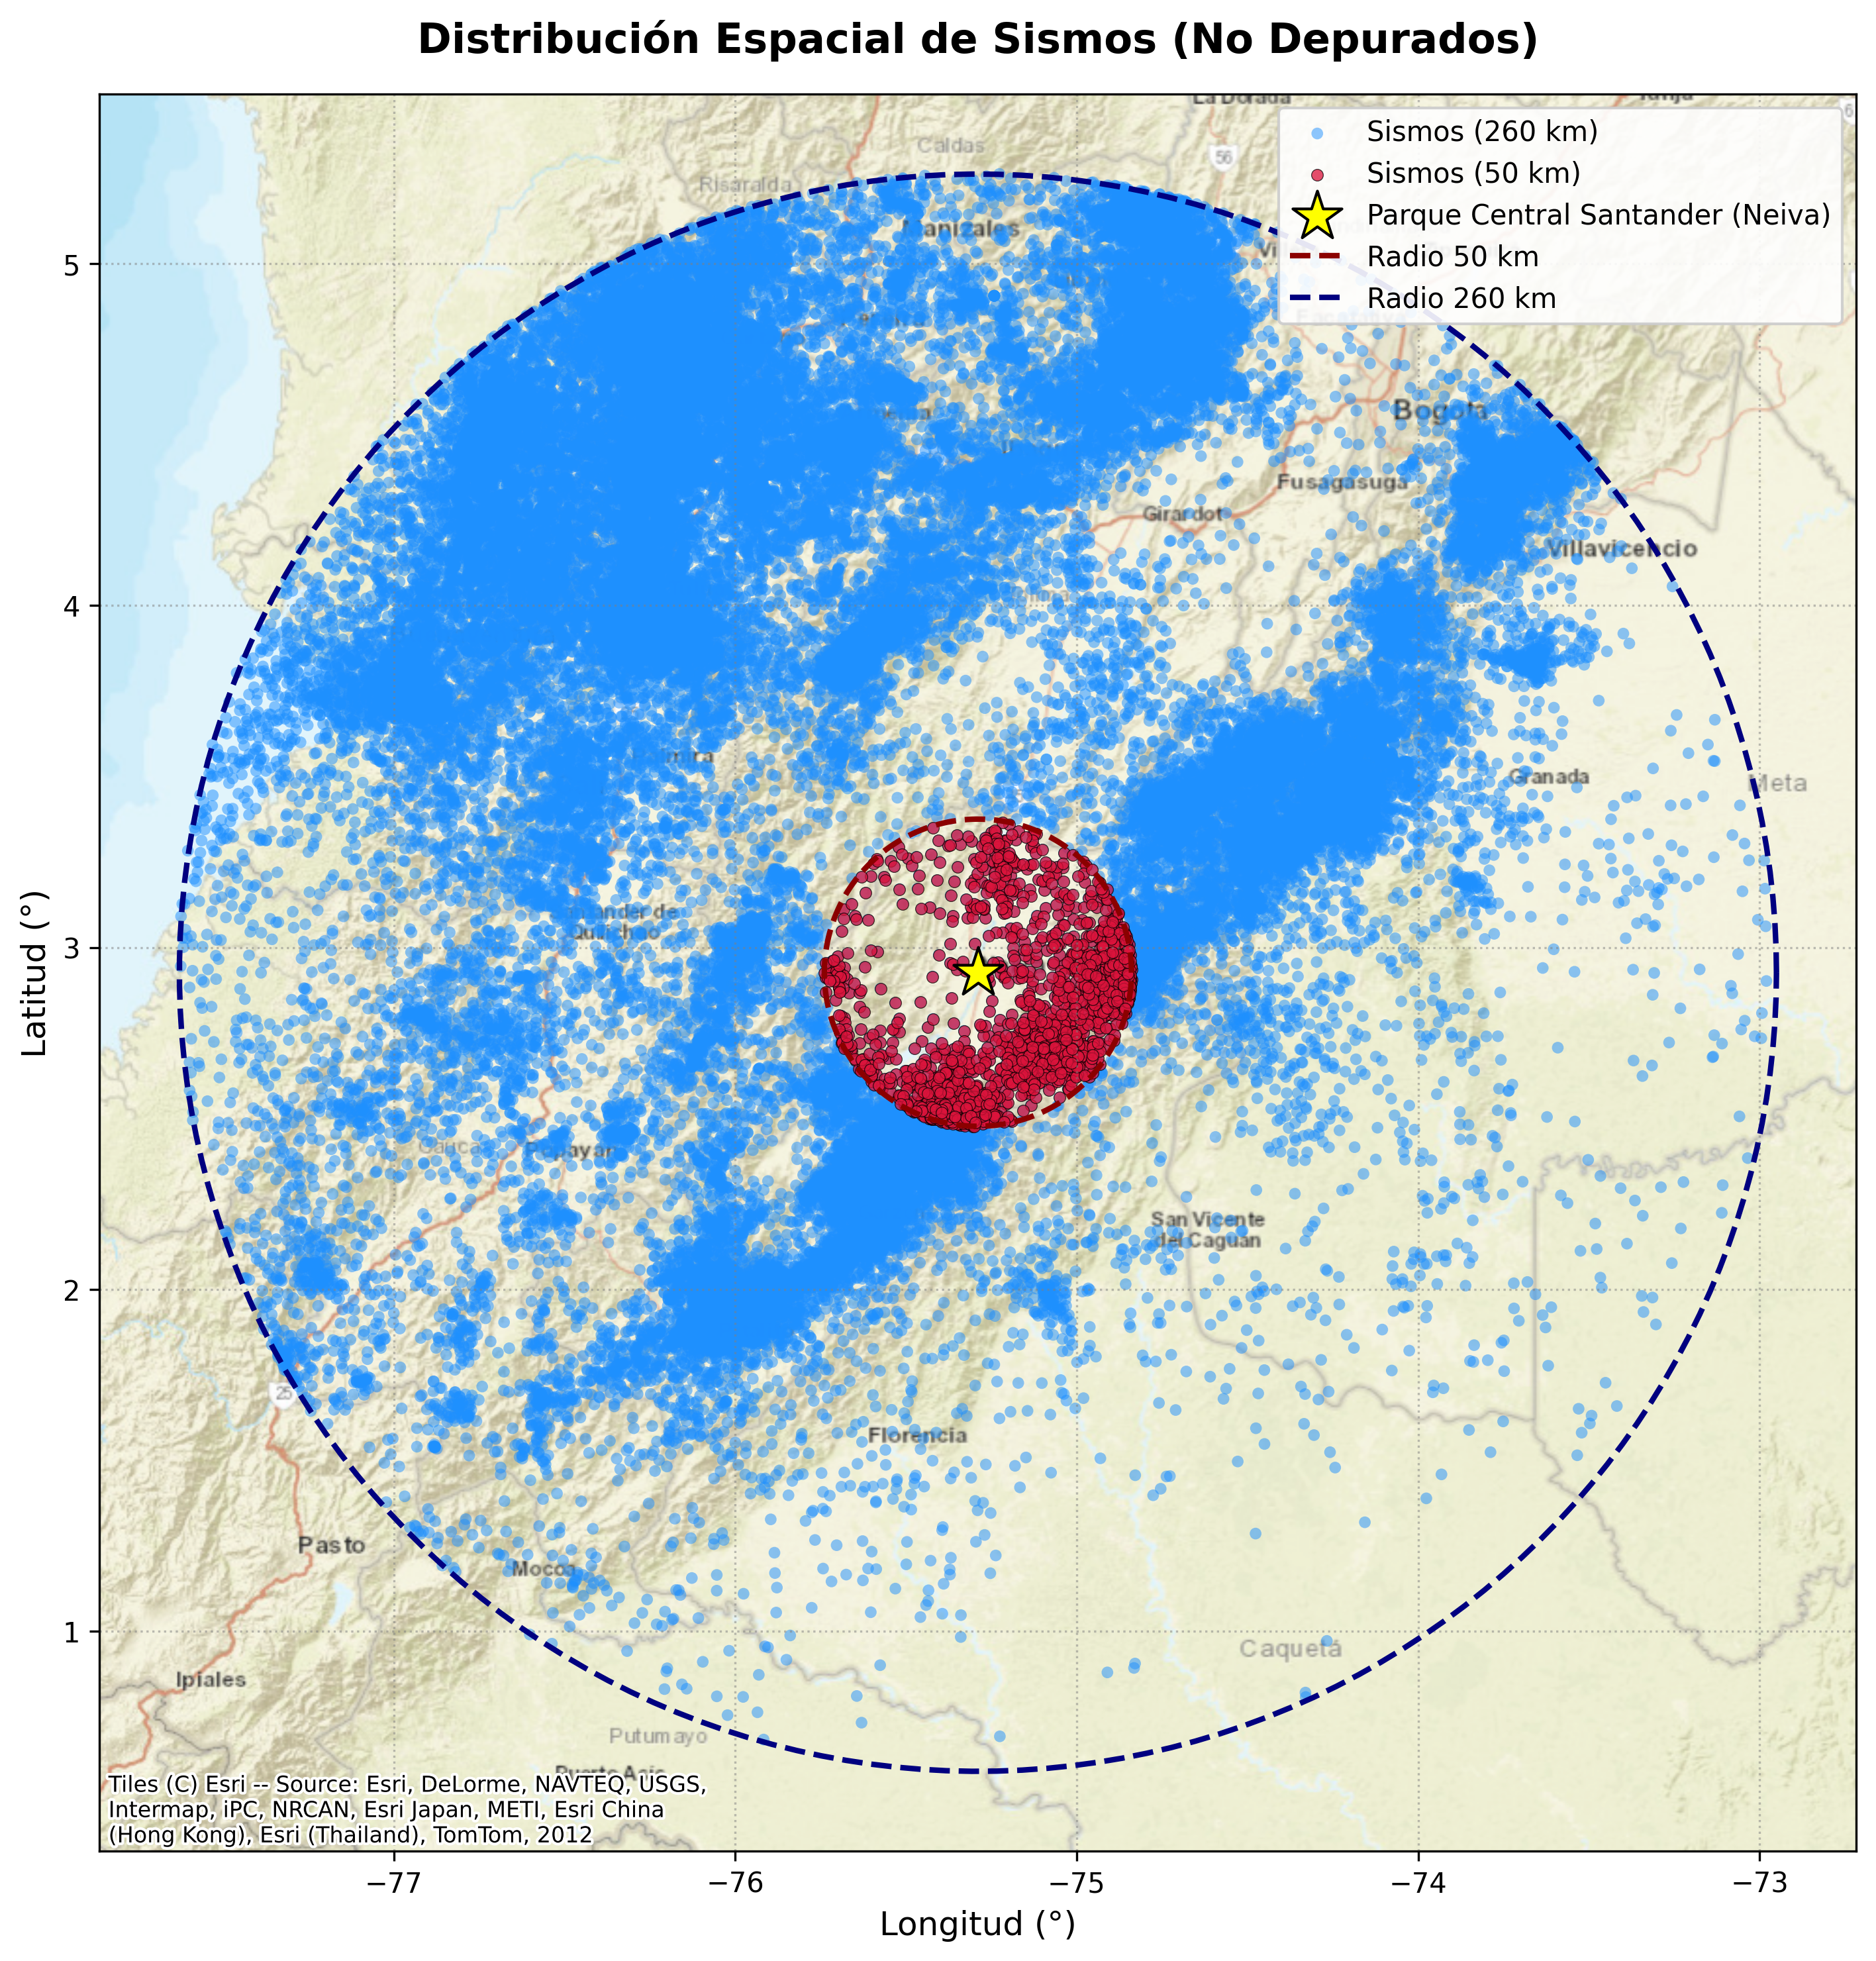
\includegraphics[width=\linewidth]{../figuras/Mapa_Sismos_No_Depurados.png}
    \caption{Catálogos combinados de entrada, sin el filtro final de magnitud ni la depuración de réplicas.}
    \label{fig:mapa-no-depurado}
\end{subfigure}\hfill
\begin{subfigure}[t]{0.485\textwidth}
    \centering
    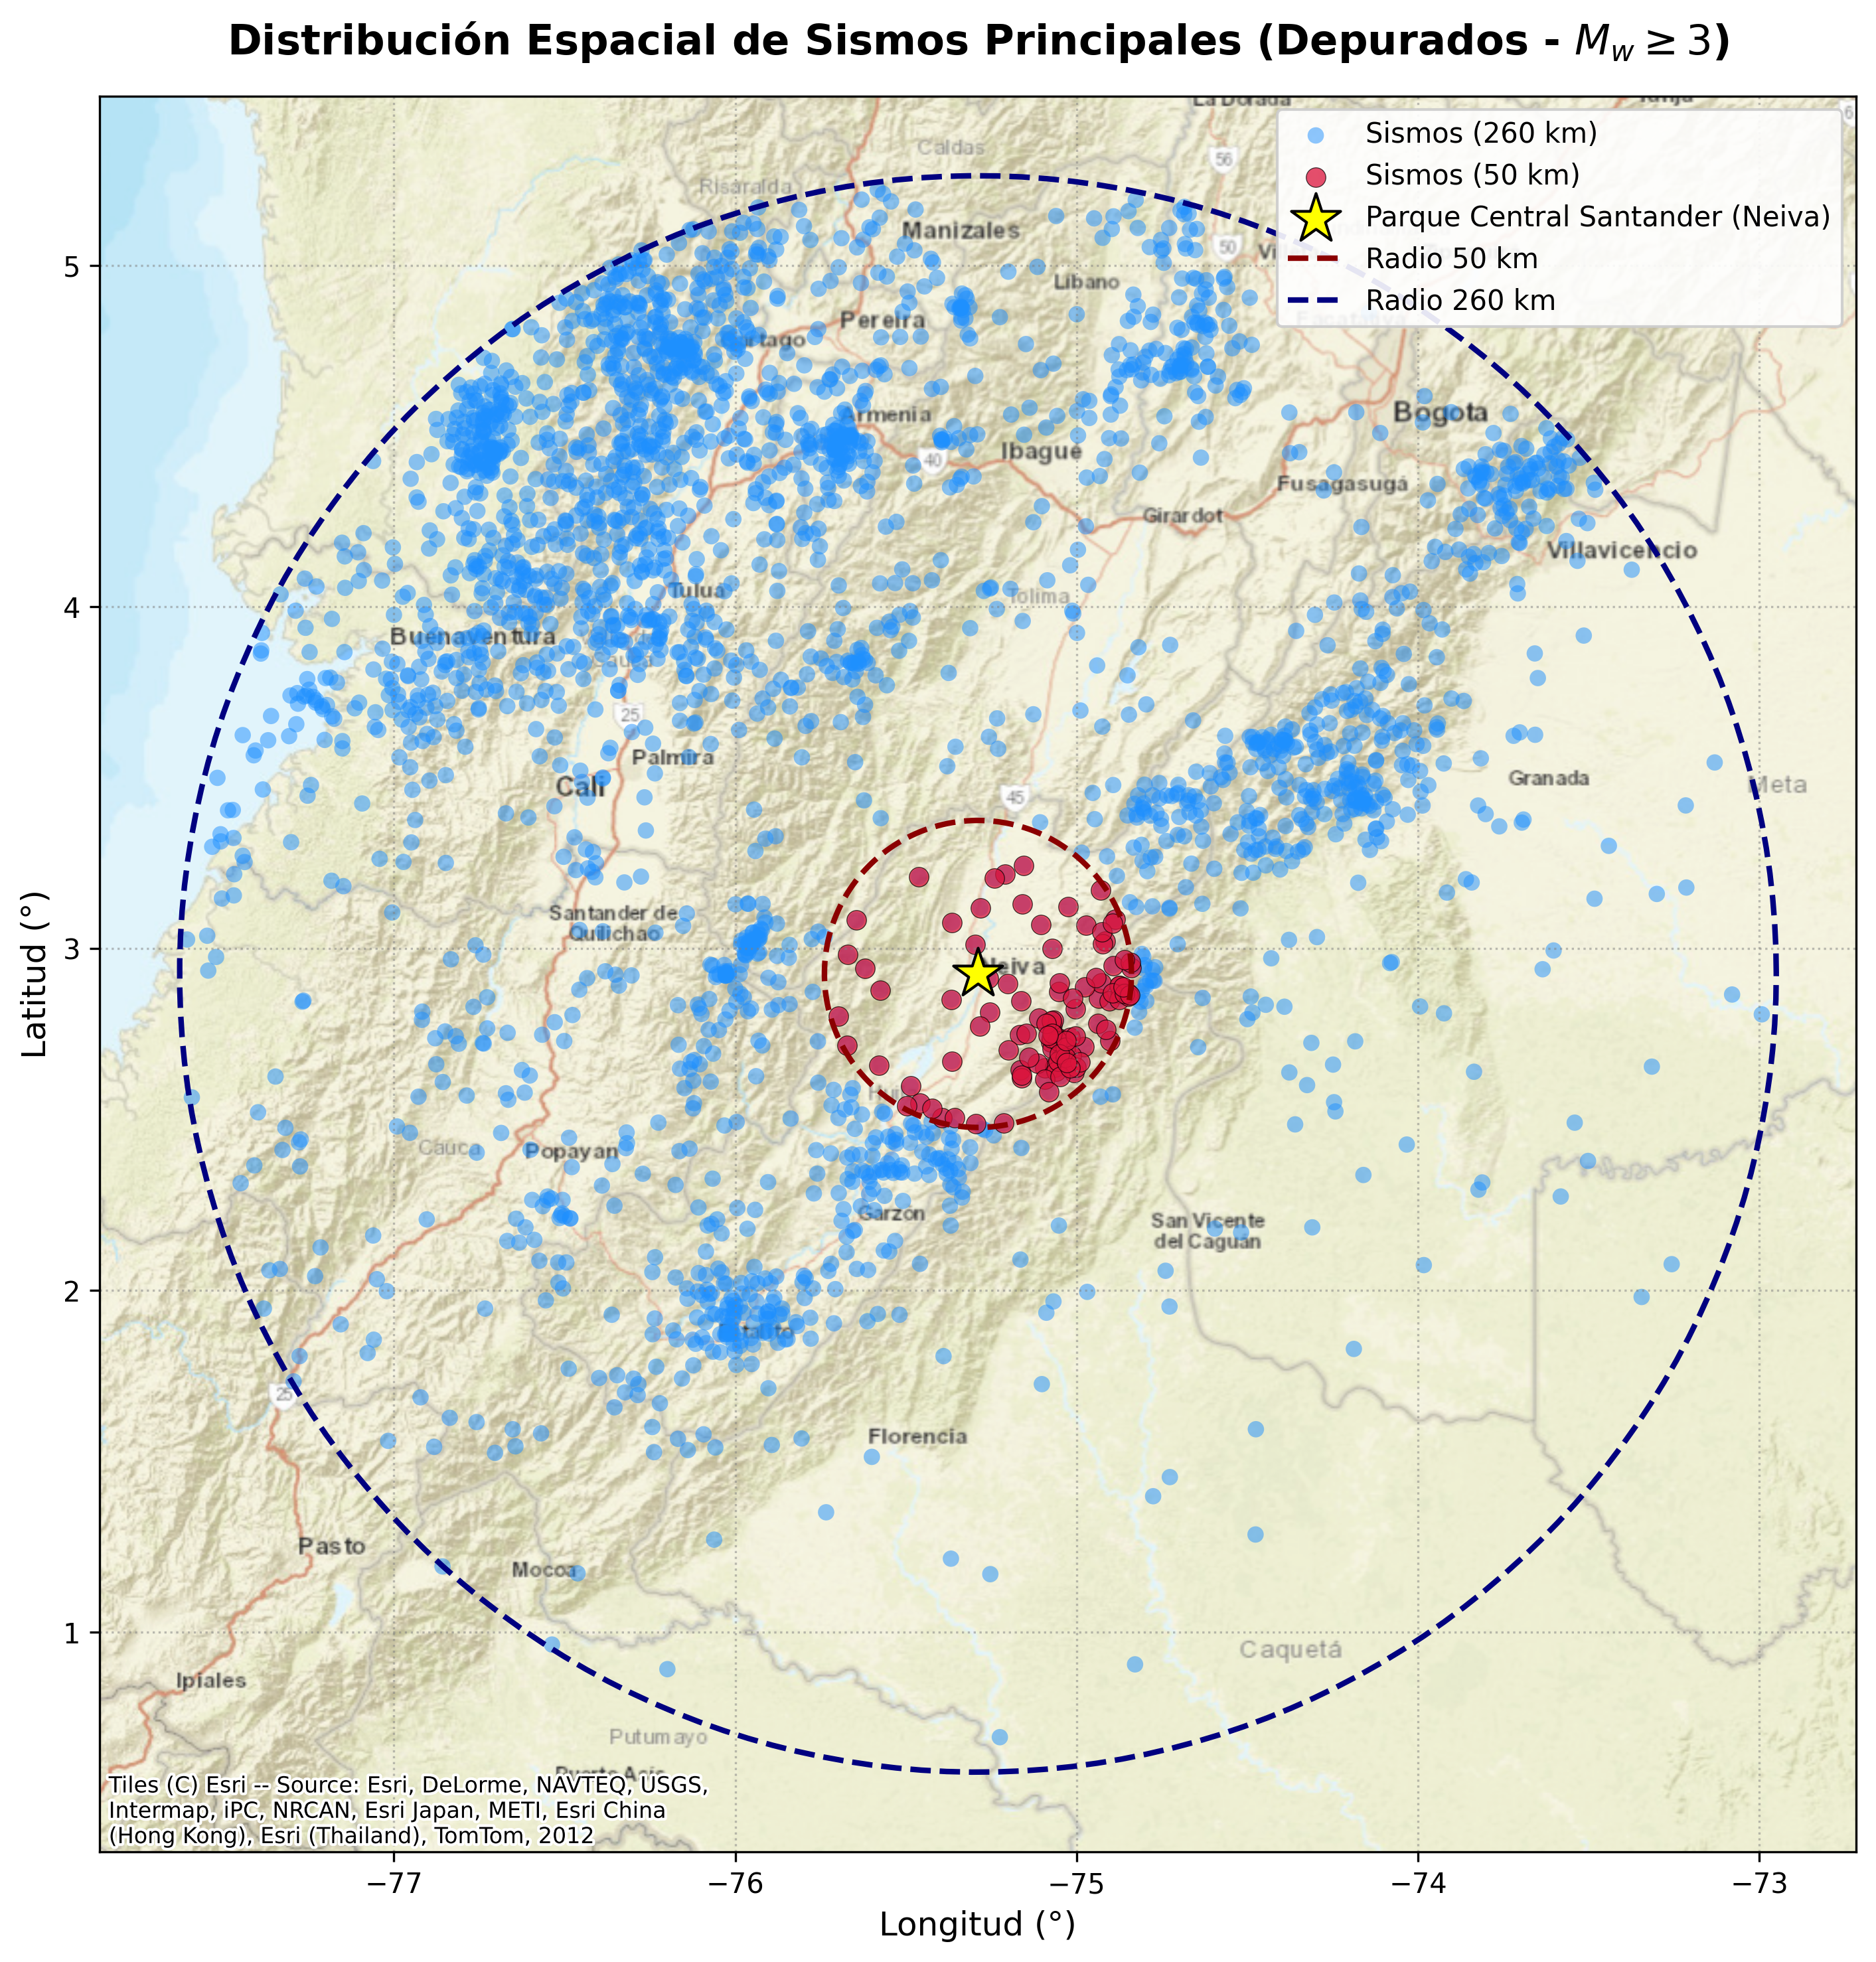
\includegraphics[width=\linewidth]{../figuras/Mapa_Sismos_Depurados.png}
    \caption{Eventos principales con $M_w\geq3$, después de la homogeneización y depuración.}
    \label{fig:mapa-depurado}
\end{subfigure}
\caption{Comparación espacial de los catálogos sísmicos de 50 y 260 km alrededor de Neiva.}
\label{fig:mapas-catalogos}
\end{figure}

\section{Estadística descriptiva de magnitudes}

La Tabla~\ref{tab:estadistica} presenta los estadísticos de los catálogos
finales con $M_w\geq3$. En los dos radios la media supera la mediana y la
asimetría es positiva, lo que indica una cola hacia magnitudes mayores. El
catálogo regional alcanza $M_w=7.4$, frente a $M_w=5.5$ en el radio local.

\begin{table}[htbp]
\centering
\caption{Estadística descriptiva de $M_w$ en los catálogos finales.}
\label{tab:estadistica}
\small
\begin{tabular}{lrrrrrrrr}
\toprule
Radio & $N$ & Media & Mediana & Desv. est. & Mín. & Máx. & Asimetría & Curtosis \\
\midrule
50 km  & 110   & 3.688 & 3.453 & 0.625 & 3.070 & 5.500 & 1.009 & 0.072 \\
260 km & 2\,627 & 3.765 & 3.500 & 0.706 & 3.000 & 7.400 & 1.273 & 1.648 \\
\bottomrule
\end{tabular}
\end{table}

La mayor asimetría y curtosis regionales reflejan una distribución más
extendida hacia magnitudes altas y la presencia de eventos extremos. Estos
estadísticos describen los registros retenidos; no corrigen sesgos por
completitud, cambios de red o incertidumbre de conversión.

\section{Relación Gutenberg--Richter}

Los ajustes Gutenberg--Richter se realizaron sobre los catálogos depurados,
desde $M_c=3.05$. En el radio de 260 km, los 33 eventos con $M_w=3.0$ forman
parte del catálogo final, pero quedan por debajo de $M_c$ y no entran en el
ajuste. Por esta razón, el tamaño de muestra regional del ajuste es menor que
el número total del catálogo.

\begin{table}[htbp]
\centering
\caption{Parámetros del ajuste Gutenberg--Richter calculados por el notebook.}
\label{tab:gutenberg-richter}
\begin{tabular}{lrrrrrr}
\toprule
Radio & $M_c$ & $N$ catálogo & $N$ ajuste & $a$ & $b$ & $R^2$ \\
\midrule
50 km  & 3.05 & 110   & 110   & 4.117 & 0.666 & 0.958 \\
260 km & 3.05 & 2\,627 & 2\,594 & 5.813 & 0.728 & 0.982 \\
\bottomrule
\end{tabular}
\end{table}

El valor de $b$ es 0.666 para 50 km y 0.728 para 260 km; ambos ajustes
presentan coeficientes de determinación altos ($R^2=0.958$ y $R^2=0.982$).
El parámetro $b$ expresa la pendiente del ajuste en el dominio de magnitudes
considerado y no debe extrapolarse sin verificar la completitud, la
independencia de los eventos y la estabilidad de la estimación.

\begin{figure}[htbp]
\centering
\begin{subfigure}[t]{0.485\textwidth}
    \centering
    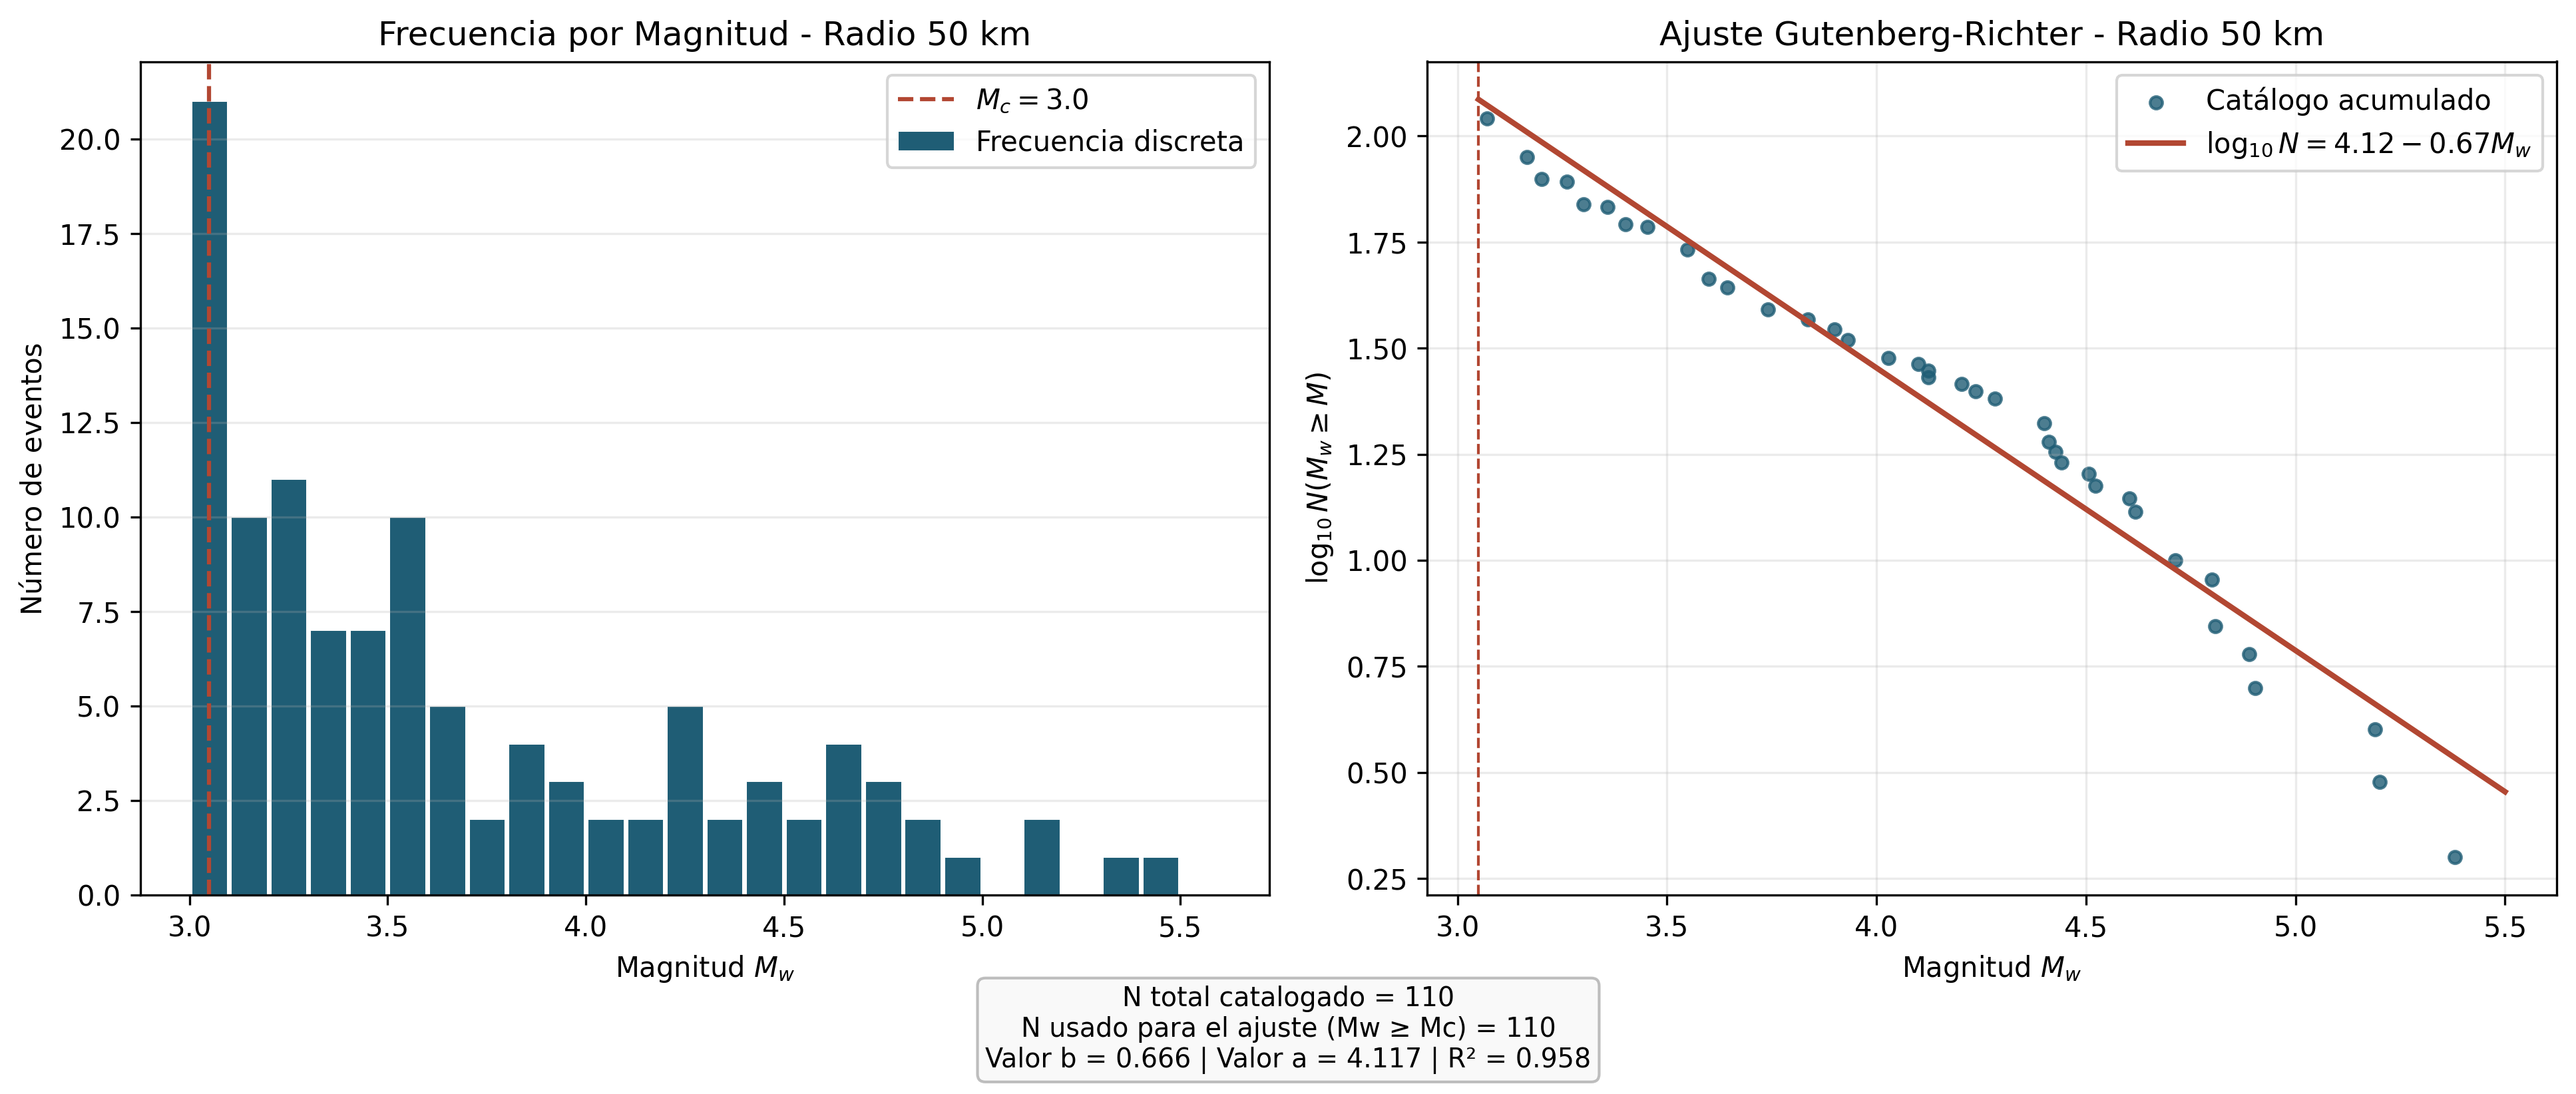
\includegraphics[width=\linewidth]{../figuras/gutenberg_richter_50km_onlymw.png}
    \caption{Radio de 50 km.}
    \label{fig:gr50}
\end{subfigure}\hfill
\begin{subfigure}[t]{0.485\textwidth}
    \centering
    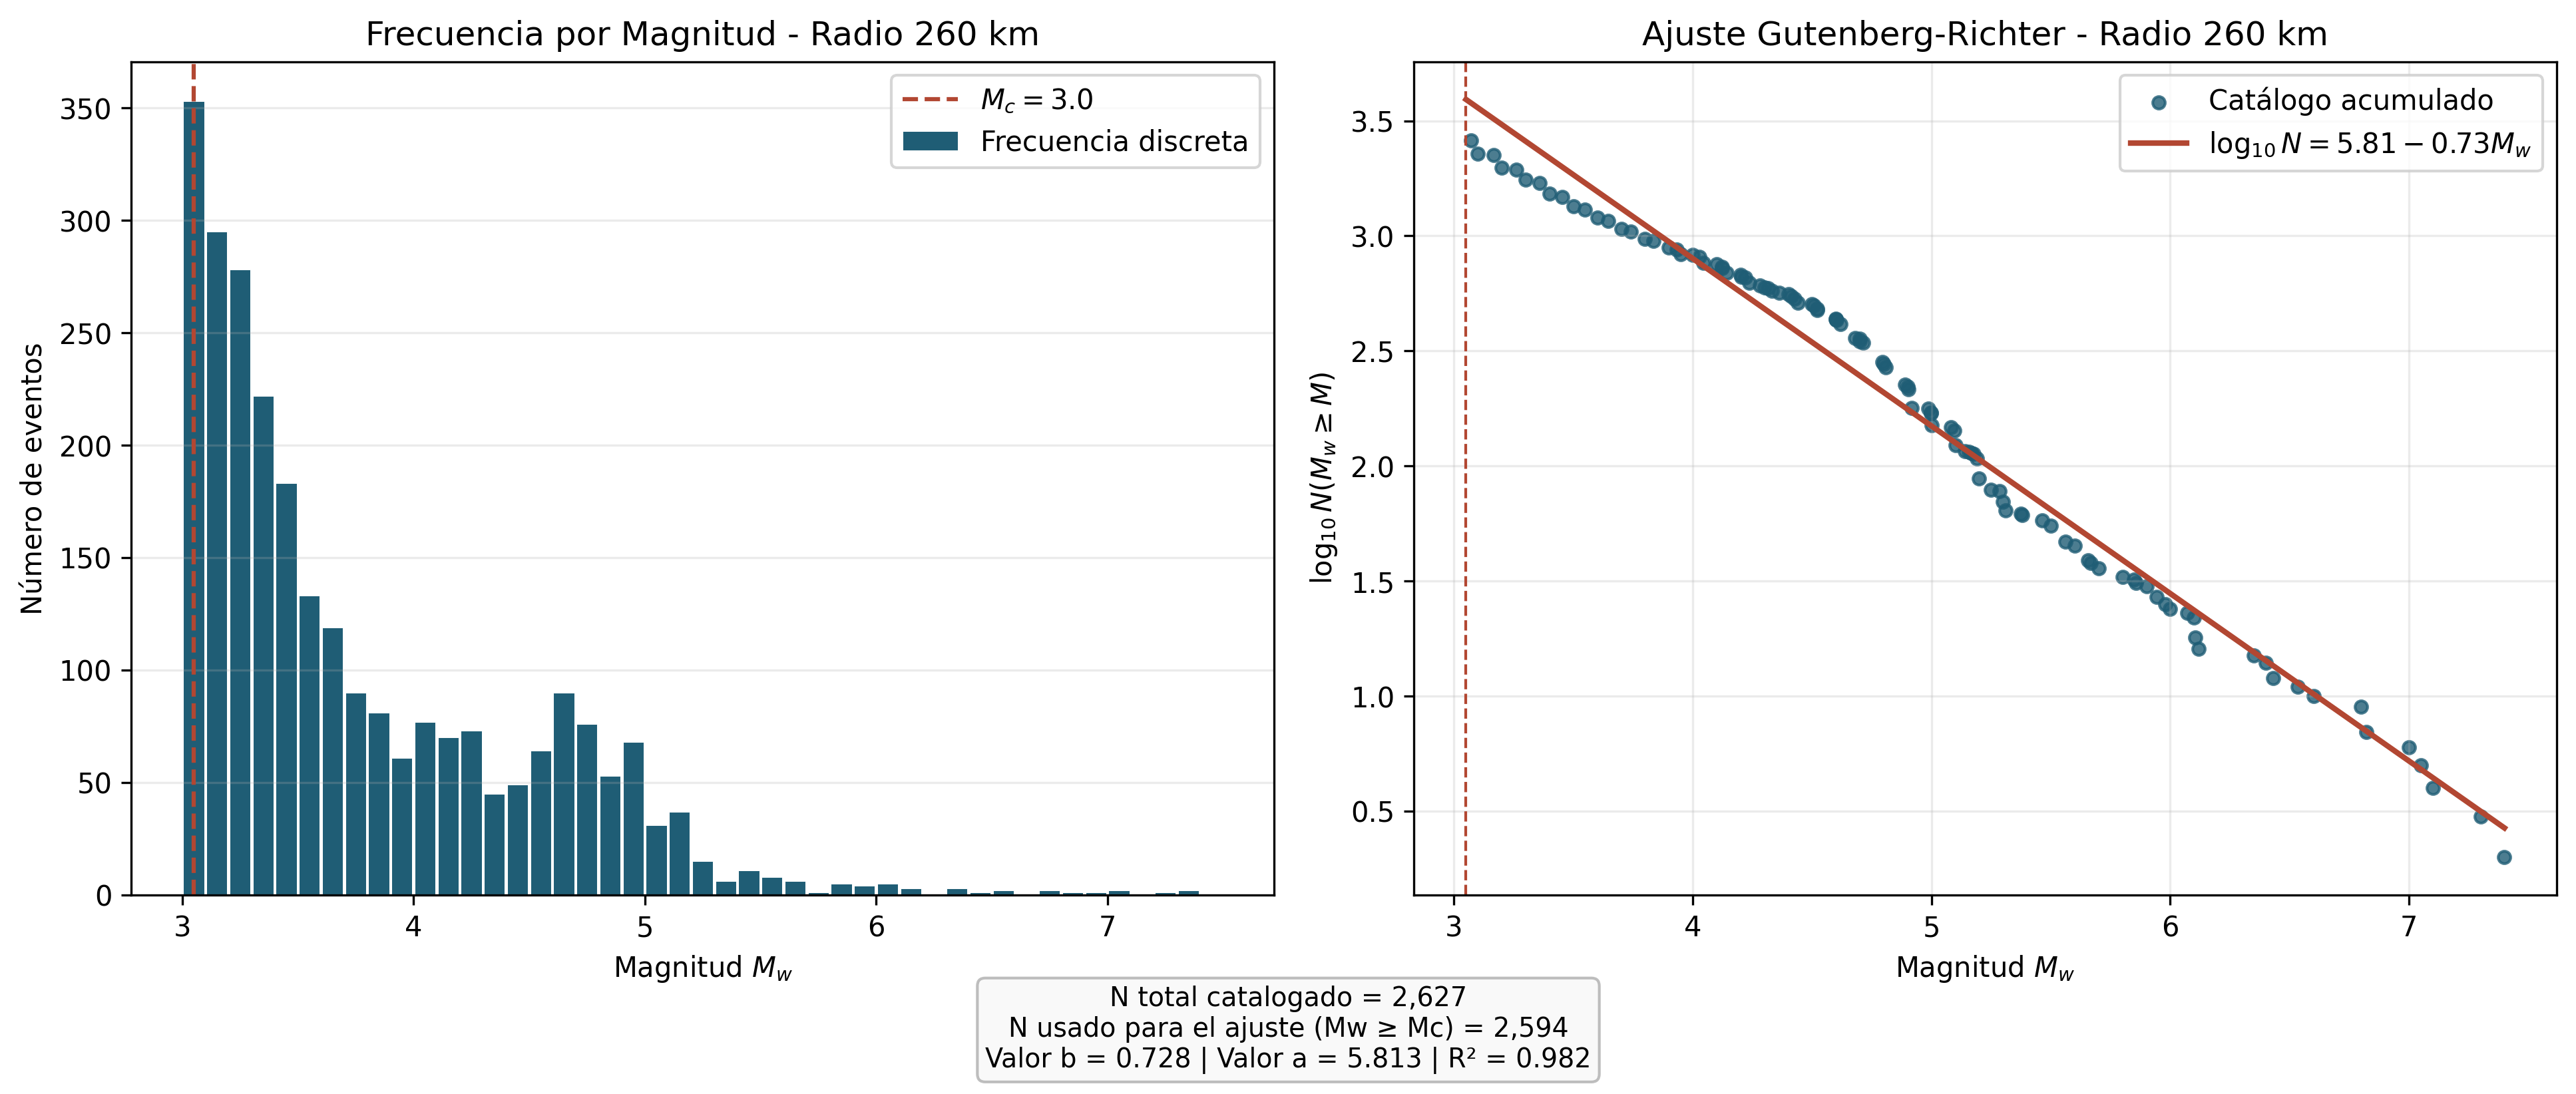
\includegraphics[width=\linewidth]{../figuras/gutenberg_richter_260km_onlymw.png}
    \caption{Radio de 260 km.}
    \label{fig:gr260}
\end{subfigure}
\caption{Frecuencia por magnitud y ajustes Gutenberg--Richter del notebook.}
\label{fig:gutenberg-richter}
\end{figure}

\chapter{Conclusiones y alcance}

\begin{enumerate}
    \item El flujo integra catálogos SGC y USGS, homogeniza las magnitudes disponibles y aplica un filtro $M_w\geq3$ junto con una regla reproducible de depuración espacio-temporal.
    \item La última ejecución retuvo 110 eventos en 50 km y 2\,627 en 260 km. El criterio implementado no eliminó eventos locales y retiró 247 candidatos regionales.
    \item Las distribuciones presentan asimetría positiva. El catálogo regional contiene la cola de magnitudes más altas y alcanza $M_w=7.4$.
    \item El análisis de recurrencia obtuvo $M_c=3.05$, con $b=0.666$ y $R^2=0.958$ para 50 km, y $b=0.728$ y $R^2=0.982$ para 260 km. En el ajuste regional se incluyeron 2\,594 de los 2\,627 eventos finales, debido al umbral $M_w\geq M_c$.
    \item Los resultados son preliminares y están condicionados por la calidad, completitud y compatibilidad de los catálogos; las conversiones empíricas y el criterio sencillo de réplicas también introducen incertidumbre.
    \item Para una evaluación de amenaza sísmica se requiere complementar este trabajo con análisis de completitud y sensibilidad, control explícito de duplicados, caracterización de sismofuentes, relaciones de movimiento fuerte y evaluación de condiciones locales, de acuerdo con el marco técnico aplicable \parencite{nsr10,sgc2018amenaza}.
\end{enumerate}

\chapter*{Referencias}
\addcontentsline{toc}{chapter}{Referencias}
\printbibliography[heading=none]

\end{document}
